% The generic preamble
\documentclass[10pt,letterpaper,fleqn,titlepage]{article}

% Define packages to use
\usepackage{natbib}
\usepackage[dvips]{graphicx,color}
\usepackage{amsmath,amssymb}
\usepackage{bm}
\usepackage{caption}
\usepackage{xr}
\usepackage{ifthen}
\usepackage[dvipdfm,colorlinks,linkcolor=blue,citecolor=blue,urlcolor=blue]{hyperref}
\usepackage{fancybox}
\usepackage{textcomp}
\usepackage{alltt}
%\usepackage{floatflt}
%\usepackage{svn}


% Redefine default page
\setlength{\textheight}{9in}  % 1" above and below
\setlength{\textwidth}{6.75in}   % 0.5" left and right
\setlength{\oddsidemargin}{-0.25in}

% Redefine default paragraph
\setlength{\parindent}{0pt}
\setlength{\parskip}{1ex plus 0.5ex minus 0.2ex}

% Define caption width and default fonts
\setlength{\captionmargin}{0.5in}
\renewcommand{\captionfont}{\sffamily}
\renewcommand{\captionlabelfont}{\bfseries\sffamily}

% Define commands for super- and subscript in text mode
\newcommand{\superscript}[1]{\ensuremath{^\textrm{#1}}}
\newcommand{\subscript}[1]{\ensuremath{_\textrm{#1}}}

% Derived commands
\newcommand{\invcm}{\textrm{cm\superscript{-1}}}
\newcommand{\micron}{\ensuremath{\mu\textrm{m}}}

\newcommand{\df}{\ensuremath{\delta f}}
\newcommand{\Df}{\ensuremath{\Delta f}}
\newcommand{\dx}{\ensuremath{\delta x}}
\newcommand{\Dx}{\ensuremath{X_{max}}}
\newcommand{\Xeff}{\ensuremath{X_{eff}}}

\newcommand{\water}{\textrm{H\subscript{2}O}}
\newcommand{\carbondioxide}{\textrm{CO\subscript{2}}}
\newcommand{\ozone}{\textrm{O\subscript{3}}}

\newcommand{\taup}[1]{\ensuremath{\tau_{#1}}}
\newcommand{\efftaup}[1]{\ensuremath{\tau_{#1}^{*}}}

\newcommand{\textbfm}[1]{\boldmath\ensuremath{#1}\unboldmath}

\newcommand{\rb}[1]{\raisebox{1.5ex}[0pt]{#1}}

\newcommand{\f}[1]{\texttt{#1}}

% Define how equations are numbered
\numberwithin{equation}{section}
\numberwithin{figure}{section}
\numberwithin{table}{section}

% Define a command for title page author email footnote
\newcommand{\email}[1]
{%
  \renewcommand{\thefootnote}{\alph{footnote}}%
  \footnote{#1}
  \renewcommand{\thefootnote}{\arabic{footnote}}
}

% Define a command to print the Office Note subheading
\newcommand{\notesubheading}[1]
{%
  \ifthenelse{\equal{#1}{}}{}
  { {\Large\bfseries Office Note #1\par}%
    {\scriptsize \sc This is an unreviewed manuscript, primarily intended for informal}\\ 
    {\scriptsize \sc exchange of information among JCSDA researchers\par}%
  }
}

% Redefine the maketitle macro
\makeatletter
\def\docseries#1{\def\@docseries{#1}}
\def\docnumber#1{\def\@docnumber{#1}}
\renewcommand{\maketitle}
{%
  \thispagestyle{empty}
  \vspace*{1in}
  \begin{center}%
     \sffamily
     {\huge\bfseries Joint Center for Satellite Data Assimilation\par}%
     \notesubheading{\@docnumber}
  \end{center}
  \begin{flushleft}%
     \sffamily
     \vspace*{0.5in}
     {\Large\bfseries\ifthenelse{\equal{\@docseries}{}}{}{\@docseries: }\@title\par}%
     \medskip
     {\large\@author\par}%
     \medskip
     {\large\@date\par}%
     \bigskip\hrule\vspace*{2pc}%
  \end{flushleft}%
  \newpage
  \setcounter{footnote}{0}
}
\makeatother
\docseries{}
\docnumber{}


% Define a command for a DRAFT watermark
\usepackage{eso-pic}
\newcommand{\draftwatermark}
{
  \AddToShipoutPicture{%
    \definecolor{lightgray}{gray}{.85}
    \setlength{\unitlength}{1in}
    \put(2.5,3.5){%
      \rotatebox{45}{%
        \resizebox{4in}{1in}{%
          \textsf{\textcolor{lightgray}{DRAFT}}
        }
      }
    }
  }
}




% Title info
\title{Validation of CRTM for Cloudy Sky Conditions Using LBLDIS}
\author{David Neil Groff\email{david.groff@noaa.gov}\\JCSDA/EMC/SAIC\\[0.25in]
        Paul van Delst\email{paul.vandelst@noaa.gov}\\JCSDA/EMC/SAIC\\[0.25in]}
\date{April, 2008}
\docnumber{??}
\docseries{CRTM}


%-------------------------------------------------------------------------------
%                            Ze document begins...
%-------------------------------------------------------------------------------
\begin{document}
\maketitle

\begin{abstract}
This report discusses work that has been done to compare CRTM and LBLDIS components for cloudy sky conditions. The proceedures used for running LBLDIS and performing the comparisons are described. Furthermore, systematic errors associated with these proceedures are described and quantified.
The LBLDIS model will be a reference for validating CRTM simulations for cloudy atmospheres. 
   
%The magnitude of the discrepancies that can be attributed to the major components of these RT models (i.e. RTSolver, LUT, Interpolation) are  The components of discrepancies between the models are attributed and analyzed.
\textbf{Keywords}: CRTM, LBLRTM, LBLDIS, Clouds  
\end{abstract}


%\section{Introduction}
%=====================

%\label{sec:intro}

\section{Running LBLDIS}
%=================
LBLDIS is a radiative transfer model that combines AER's line by line radiative transfer model (LBLRTM) and the discrete ordinate radiative transfer model (DISORT) and is able to compute radiances
for scattering atmospheres. The LBLDIS model requires the following inputs: LBLDIS formatted parameter files, 
LBLRTM optical depth output, and the atmospheric layering and structure information used by the 
LBLRTM. A further description of these inputs are provided in the following subsections.

\subsection{LBLRTM Calculations}
The LBLRTM performs gas absorption computations and is run externally to LBLDIS.
To run the LBLRTM it is necessary to first create TAPE5 files that specify the level quantities
of the profile data to be used for running the LBLRTM. In this project CRTM atmosphere layer data was converted to level data in
order to create TAPE5 files. Linear extrapolation is performed to obtain the surface level quantities 

\begin{equation}
level(1) = layer(1) - ((layer(2) - layer(1))/2)
\end{equation}          

and a simple averaging scheme is used to obtain the level quantities from level k=2 to the top of the atmosphere. 

\begin{equation}
level(k) = (layer(k) + layer(k+1)/2)
\end{equation}

The LBLRTM calculates layer atmosphere quantities using the level atmosphere quantities provided in the TAPE5 files. The LBLRTM calculated layer atmosphere quantities are included in TAPE7 files and are used by the LBLRTM to perform the gas computations.
In addition to providing the level profile quantities the TAPE5 file is used to specify the wavenumber (cm\superscript{-1}) range and view geometry for the LBLRTM calculations. For the initial results presented in this report the wavenumber range has been set to span the spectral response functions for hirs4\textunderscore{}n18 channels 1-19 and the view geometry has been set to nadir. 



%TAPE7 atmospheric data files are generated by running the LBLRTM with the TAPE5 input files.  These files provide the layer information used to perform LBLRTM gas computations.
%Data from these TAPE7 files will 
%be used to create the CRTM atmosphere file . The impact of the atmospheric layering conversions on the CRTM calculations is discussed in section2.
%Therefore, in order to run the LBLRTM for a CRTM atmosphere file the CRTM layer
%data is first converted to level quantities. 
%\end
   

%The TAPE5 MUNITS option can be set to 1 or 0 with corresponding absorber units of ppv or number density (\#/cm\superscript{2}). The CRTM absorber units are ppmv for ozone and mixing 
%ratio (g/kg) for water vapor. Therefore, when MUNITS is set to 1 the number of conversions necessary to fill the CRTM atmosphere structure with TAPE7 LBLRTM ouput is reduced. 
%In this work the view geometry has been set to nadir. The wavelength ranges are set to encompass the spectral response functions for hirs418 channels. The LBLRTM produces atmospheric
%layering information (TAPE7 files) and layer optical depth data which is necessary input for running LBLDIS.

%\subsection{}

\subsection{LBLDIS Parameter Files}
Parameter files needed to run the LBLDIS provide the cloud data, surface data, view geometry, wavenumber specifications (range and spacing), a path to cloud optical property look up table (LUT) data and a path to the LBLRTM output data. For accurate comparisons between the LBLDIS and CRTM models it is necessary to set the aforementioned
parameters to match the parameters used when running the CRTM (i.e surface emissivity and surface temperature).  
Other than the cloud density information all data in the parameter files can be set to exactly match specifications used when running the CRTM. The absolute mass content for clouds provided in CRTM atmosphere files has to be converted to relative number density units as required by the LBLDIS model.
To do this the absolute layer density in units of (kg/m\superscript{2}) is first divided by the layer thickness to obtain a relative mass density. The relative cloud mass density is then converted to a relative number density by dividing out the mass of each droplet (assuming an intrinsic water density of 1000.0 kg/m\superscript{3}).  
For clear sky comparisons between LBLDIS and CRTM the clouds are removed from the LBLDIS parameter files. 


%Note that the absolute mass content data for clouds provided in CRTM atmosphere files was converted to relative number density units of (\#/m\superscript{3}) that are needed to run LBLDIS.
%\ref{fig:Parameter_Example} is an example of a LBLDIS parameter file with a short description of the information provided in each line. 
%\subsection{}
%\section{}

\section{Systematic Errors From Atmosphere Conversions}
%The previously described Layer to level (level to layer) atmosphere conversions needed to create TAPE5 LBLRTM files introduce systematic errors in LBLDIS versus CRTM comparisons. That is 

\subsection{Atmosphere Files}
There are inconsistincies between the CRTM atmosphere data used to create the TAPE5 files and the TAPE7 file that specifies the atmosphere layer data for the LBLRTM gas
absorption computations. The layer to level conversions needed to create the LBLRTM TAPE5 files and the level to layer conversions performed by the LBLRTM that produce the layer information used in the LBLRTM gas computations are the sources for these inconsistincies. To quantify the impact of these inconsistincies on CRTM BT calculations three new CRTM atmosphere files were created using TAPE7 data. The impact on CRTM brightness temperature calculations is discussed in section 3.

The three new CRTM atmosphere files will hereafter be referred to as A1, A2 and A3. The A1 file contains absorber amount data from the original CRTM file, but the pressure and temperature information in this file has been extracted from the LBLRTM TAPE7 files. Files A2 and A3 contain temperature, pressure and absorber amount data extracted from the TAPE7 files. The only distinction between the A2 and A3 data files is that the A2 file absorber amounts were extracted from TAPE7 files that contained absorber column densities in units of (molecules/cm\superscript{2}) whereas the A3 absorber amount data was extracted from TAPE7 files that contained abosrber mixing ratios in (ppv). Data from the original file used to create the TAPE5 files is hereafter referred to as A0. The plots in \ref{fig:Differences_Tropical}, \ref{fig:Differences_Midlatitude_summer}, \ref{fig:Differences_Subarctic_summer}, and \ref{fig:Differences_Subarctic_winter} show differences of temperature, pressure and absorber amount between data extracted from the LBLRTM TAPE7 files and data from A0 for Tropical, Subarctic summer, Subarctic winter and Midlatitude summer profiles. Temperature and pressure differences for the four profile climatologies shown are much less than 1 percent up to around 10hPa. Water vapor and Ozone amount differences are greater than 1 percent for a significant portion of layers below 10hPa. %The data above 10hPa is sparse so the differences shown above this altitude are not representative. %Differences resulting from units conversions shown in the A3 versus A2 absorber amount comparison plots are small relative to the A3 (LBLRTM TAPE7) versus A0 (Original CRTM file) absorber amount differences.   

The percent differences in absorber amounts between the A2 and A3 file data demonstrate that discrepancies attributed to units conversions are small relative to the differences between A3 (TAPE7 LBLRTM data) and A0 (Original CRTM data) absorber amounts for layers below 10hPa. The absorber data above 10hPa is sparse, therefore differences above this altitude are relatively insignificant. 

%These plots demonstrate that temperature and pressure differences between the TAPE7 and A0 data are predominately less than 1 percent. However, water vapor and Ozone amount differences between the data in the files is frequently larger than 2 percent. Comparisons between A3 and A2 absorber amounts indicate that the absorber amount conversions that produce the data for these files resulted in slightly different absorber amounts. Discrepancies produced from the absorber amount conversions are an order of magnitude smaller than the differences associated with the layer to level and (level to layer) conversions. 

  %(plots. Absorber amount
%differences between the original data file contained in A1 and TAPE7 data contained in A3 are predominately less than 2 percent. Differences in absorber amounts between A2 and A3 demonstrate that some error is introduced in converting units (although this differences is small).  

%  cA file denoted as A1 in figure 1 contains CRTM temperature and pressure data
%that was extracted from TAPE7 pressure and temperature data. A second file denoted as A2 in figure 1 contains CRTM temperature, pressure and absorber 
%amount (H2O and OZO) data that was extracted from a TAPE7 data file that contained number density (/cm) absorber amounts. The A2 CRTM file absorber amounts had to be converted to CRTM units using the (KMOLpmv) and (ppmvR) utility available in the CRTM. A third file denoted as A3 in figure 1 contains
%CRTM temperature, pressure and absorber amount (H2O and OZO) data that was extracted from a TAPE7 data file that contained ppv absorber amounts. The plots
%in figure 1 demonstrate that the differences in pressure and temperature associated with the atmosphere conversions resulted in percentage differences
%of less than 1. Although the absorber amounts were modified to more accurately represent the TAPE7 data the plots in figure 1 demonstrate that
%some error was introduced by using the conversion utilities. 

\begin{figure}[htp]
  \centering{}
  \includegraphics[scale=0.8]{./graphics/Atmosphere_Differences_08.eps}
  \caption{Plots of differences between TAPE7 atmosphere data and CRTM atmosphere data
  that was originally used to create the LBLRTM TAPE5 files for a Tropical profile climatology}
  \label{fig:Differences_Tropical}
\end{figure}

\begin{figure}[htp]
  \centering{}
  \includegraphics[scale=0.8]{./graphics/Atmosphere_Differences_01.eps}
  \caption{Plots of differences between TAPE7 atmosphere data and CRTM atmosphere data
  that was originally used to create the LBLRTM TAPE5 files for a Midlatitude summer profile climatology}
  \label{fig:Differences_Midlatitude_summer}
\end{figure}

\begin{figure}[htp]
  \centering{}
  \includegraphics[scale=0.8]{./graphics/Atmosphere_Differences_14.eps}
  \caption{Plots of differences between TAPE7 atmosphere data and CRTM atmosphere data
  that was originally used to create the LBLRTM TAPE5 files for a SubArctic summer profile climatology}
  \label{fig:Differences_Subarctic_summer}
\end{figure}

\begin{figure}[htp]
  \centering{}
  \includegraphics[scale=0.8]{./graphics/Atmosphere_Differences_15.eps}
  \caption{Plots of differences between TAPE7 atmosphere data and CRTM atmosphere data
  that was originally used to create the LBLRTM TAPE5 files for a Subarctic winter profile climatology}
  \label{fig:Differences_Subarctic_winter}
\end{figure}



%\begin{figure}[htp]
%  \centering{}
%  \includegraphics[scale=0.8]{./graphics/BT_Diffs_01.eps}
%  \caption{Plots of BT simulation differences}
%  \label{fig:Simulation_Differences}
%\end{figure}

%\subsection{}

\subsection{Impact of Atmosphere Differences on CRTM BT's}

The plots in \ref{fig:BT_Differences_Tropical}, \ref{fig:BT_Differences_Midlatitude_summer}, \ref{fig:BT_Differences_Subarctic_summer} and \ref{fig:BT_Differences_Subarctic_winter} 
represent clear sky comparisons between the CRTM and LBLDIS, and the impact of the previously described atmosphere differences on clear sky CRTM brightness temperature (BT) simulations for Tropical, Subarctic Summer, Subarctic Winter and Midlatitude Summer profiles. The LBLDIS result was obtained by convolving radiances at .1cm\superscript{-1} resolution with hirs4\textunderscore{}n18 spectral response functions. All results shown in this initial report are for hirs4\textunderscore{}18 channels 1-19 at nadir.

In the case of the Tropical, Subarctic winter and Midlatitude summer climatology profiles the impact of atmosphere differences between A3 and A0 are less than 0.1K. In the case of the Subarctic summer profile the impact of the atmosphere differences between A3 and A0 is greater than 0.1K and less than 0.3K for several channels. For all cases the differences between A3 and A2 CRTM simulations are less than 0.01 K. The A3 versus A2 comparisons are reasonably indicative of differences between LBLDIS and A3\textunderscore{}CRTM simulations that can be attributed to systematic error, because they are representative of discrepancies associated with absorber amount unit conversions. The results also indicate that the maximum differences between LBLDIS and CRTM simulations are four orders of magnitude larger than the differences between A3 and A2 CRTM simulations. 




%can be attributed to atmosphere differences. That is the LBLDIS atmosphere and A3 only differ by discrepancy associated with absorber amount conversions. 
%
%The impact of the absorber amount conversions is four orders of magnitude smaller than the model differences.  
%
%That is the only differences between A3 and A2 are the type of unit conversions that were used to convert TAPE7 absorber amount units to CRTM absorber amount units.
%
%
%reflect the amount of difference between LBLDIS and CRTM simulations that can
%be attributed to atmosphere differences. 

%is about two orders of magnitude smaller than differences between the LBLDIS and CRTM. For the Subarctic Summer profile the impact of the amtosphere changes is greater than 0.1K for several of the channels and this impact is similar in magnitude       

\begin{figure}[htp]
  \centering{}
  \includegraphics[scale=0.8]{./graphics/BT_Differences_08.eps}
  \caption{Plots showing LBLDIS versus CRTM clear sky brightness temperature comparisons and the
  impact of the atmosphere differences on CRTM brightness temperature simulations. These plots were 
  made from Tropical profile simulations.}
  \label{fig:BT_Differences_Tropical}
\end{figure}

\begin{figure}[htp]
  \centering{}
  \includegraphics[scale=0.8]{./graphics/BT_Differences_01.eps}
  \caption{Plots showing LBLDIS versus CRTM clear sky brightness temperature comparisons and the
  impact of the atmosphere differences on CRTM brightness temperature simulations. These plots were 
  made from Midlatitude summer simulations.}
  \label{fig:BT_Differences_Midlatitude_summer}
\end{figure}

\begin{figure}[htp]
  \centering{}
  \includegraphics[scale=0.8]{./graphics/BT_Differences_14.eps}
  \caption{Plots showing LBLDIS versus CRTM clear sky brightness temperature comparisons and the
  impact of the atmosphere differences on CRTM brightness temperature simulations. These plots were 
  made from Subarctic summer simulations.}
  \label{fig:BT_Differences_Subarctic_summer}
\end{figure}

\begin{figure}[htp]
  \centering{}
  \includegraphics[scale=0.8]{./graphics/BT_Differences_15.eps}
  \caption{Plots showing LBLDIS versus CRTM clear sky brightness temperature comparisons and the
  impact of the atmosphere differences on CRTM brightness temperature simulations. These plots were 
  made from Subarctic winter simulations.}
  \label{fig:BT_Differences_Subarctic_winter}
\end{figure}

%\begin{figure}[htp]
%  \centering{}
%  \includegraphics[scale=0.8]{./graphics/BT_Diffs_01.eps}
%  \caption{Plots of BT simulation differences}
%  \label{fig:BT_Simulation_Differences}
%\end{figure}

%The plots in figure 2 demonstrate that LBLDIS versus CRTM errors introduced by atmosphere conversions are less than .1K. This difference is much smaller than the differences between
%LBLDIS and the CRTM. 
%
%The file A0 represents the initial
%CRTM file that was used to create the LBLRTM TAPE5 files. The errors introduced by atmosphere conversions are small commpared to the CRTM versus LBLDIS BT differences for the A0 file. 

%\section{}

\section{LBLDIS Versus CRTM Clear Sky Components}

For clear sky calculations the differences between LBLDIS and CRTM are the additive effects of the gas absorption computations and the solving of the radiative transfer equation. To isolate  differences associated with gas absorption computations the CRTM radiative transfer equation is run with LBLRTM optical depth data at instrument resolution. The LBLRTM optical depth data at instrument resolution is obtained by convolving LBLRTM TAPE20 transmittance profile data to instrument resolution. Before running the CRTM's radiative transfer solver the instrument resolution LBLRTM transmittances are converted to optical depths. The result of running the LBLRTM instrument resolution optical depths through the CRTM's radiative transfer solver will hereafter be referred to as CRTM(TauProfile). The plots in \ref{fig:Clear_Sky_Tropical}, \ref{fig:Clear_Sky_Midlatitude_summer}, \ref{fig:Clear_Sky_Subarctic_winter} and \ref{fig:Clear_Sky_Subarctic_summer} show brightness temperature comparisons between the LBLDIS, CRTM and CRTM(TauProfile) calculations for Tropical, Subarctic summer, Subarctic winter and Midlatitude summer. The comparisons between LBLDIS and CRTM(TauProfile) are representative of the clear sky differences between LBLDIS and CRTM that can be attributed to the solvers of the radiative transfer equation used by the 
respective models. The results indicate that differences between LBLDIS and CRTM(TauProfile) are much less than 0.1K for channels 1-16.
The absolute value of the differences between LBLDIS and CRTM(TauProfile) for channels 17, 18 and 19 are greater than 2K for all profile climatologies shown. From channel 17 to channel 19 the differences between LBLDIS and CRTM(TauProfile) increase with channel number. The gas absorption differences represented by the green plots contribute to nearly all the differences exhibited in the LBLDIS and CRTM comparisons for channels 1-16. The maximum gas absorption differences occur at channel 17. For channels 17-19 differences attributed to the radiative transfer solvers and gas absorption computations somewhat offset each other in the LBLDIS versus CRTM comparison results. 

For most channels the gas absorption differences are significantly larger for the Midlatitude summer and Tropical profiles than for the Subarctic profiles. This suggest that the handling of water vapor for the low peaking channels may be significantly contributing to the gas absorption differences between the models. This is particularly evident for hirs4\textunderscore{}n18 channel number 8. \ref{fig:Transmittances_Tropical_ch8} and \ref{fig:Transmittances_Subarctic_ch8} demonstrate that differences in layer transmittances
between CRTM(TauProfile) and CRTM are only realized in the presence of water vapor. The transmittance differences are more substantial for the tropical profile, because the amount
of water vapor in the troposphere is an order of magnitude larger than for the Subarctic winter profile. 

The large channel 17 differences that are seen in all profiles are perhaps more associated with a combination of factors. The plots in \ref{fig:Transmittances_Tropical_ch17} and \ref{fig:Transmittances_Subarctic_ch17} demonstrate that channel 17 transmittance differences are apparent even for layers with little to no water vapor above 100hPa. 

%as CO\superscript{2} absorption decreases
\begin{figure}[htp]
  \centering{}
  \includegraphics[scale=0.8]{./graphics/Clear_Sky_Comparison_08.eps}
  \caption{Plots of differences between LBLDIS, CRTM and CRTM(TauProfile) calculated brightness temperatures for
   a Tropical atmosphere.}
  \label{fig:Clear_Sky_Tropical}
\end{figure}

\begin{figure}[htp]
  \centering{}
  \includegraphics[scale=0.8]{./graphics/Clear_Sky_Comparison_01.eps}
  \caption{Plots of differences between LBLDIS, CRTM and CRTM(TauProfile) calculated brightness temperatures for
   a Midlatitude summer atmosphere.}
  \label{fig:Clear_Sky_Midlatitude_summer}
\end{figure}

\begin{figure}[htp]
  \centering{}
  \includegraphics[scale=0.8]{./graphics/Clear_Sky_Comparison_14.eps}
  \caption{Plots of differences between LBLDIS, CRTM and CRTM(TauProfile) calculated brightness temperatures for
   a Subarctic summer atmosphere.}
  \label{fig:Clear_Sky_Subarctic_summer}
\end{figure}

\begin{figure}[htp]
  \centering{}
  \includegraphics[scale=0.8]{./graphics/Clear_Sky_Comparison_15.eps}
  \caption{Plots of differences between LBLDIS, CRTM and CRTM(TauProfile) calculated brightness temperatures for
   a Subarctic winter atmosphere.}
  \label{fig:Clear_Sky_Subarctic_winter}
\end{figure}

\begin{figure}[htp]
  \centering{}
  \includegraphics[scale=0.8]{./graphics/Transmittance_Comparison_ch08_P08.eps}
  \caption{Transmittances and transmittance differences for hirs4 n18 channel 8. The plots also show the absorber amounts
  for the tropical profile.} 
  \label{fig:Transmittances_Tropical_ch8}
\end{figure}

\begin{figure}[htp]
  \centering{}
  \includegraphics[scale=0.8]{./graphics/Transmittance_Comparison_ch08_P15.eps}
  \caption{Transmittances and transmittance differences for hirs4 n18 channel 8. The plots also show the absorber amounts
  for the Subarctic profile.}
  \label{fig:Transmittances_Subarctic_ch8}
\end{figure}

\begin{figure}[htp]
  \centering{}
  \includegraphics[scale=0.8]{./graphics/Transmittance_Comparison_ch17_P08.eps}
  \caption{Transmittances and transmittance differences for hirs4 n18 channel 17. The plots also show the absorber amounts
  for the Tropical profile.}
  \label{fig:Transmittances_Tropical_ch17}
\end{figure}

\begin{figure}[htp]
  \centering{}
  \includegraphics[scale=0.8]{./graphics/Transmittance_Comparison_ch17_P15.eps}
  \caption{Transmittances and transmittance differences for hirs4 n18 channel 17. The plots also show the absorber amounts
  for the Subarctic profile.}
  \label{fig:Transmittances_Subarctic_ch17}
\end{figure}





%%A comparison between this result and conventional CRTM calculations for the A3 atmosphere are representative of gas absorption differences between LBLDIS and the CRTM.

%The components that contribute to the LBLDIS and CRTM clear sky simulations are the respective solvers for the radiative transfer equation and 
%
%The clear sky simulation comparisons between the LBLDIS and CRTM models provide a validation tool for the CRTM's solver of the radiative
%transfer equation and the CRTM's handling of gas absorption. To isolate the difference associated with gas absorption computations the CRTM radiative transfer equation is run with LBLRTM optical depth data at instrument resolution. The LBLRTM optical depth data was  
%
%LBLDIS gas absorption is computed by the LBLRTM. The gas absorption component of the differences between LBLDIS and CRTM can be calculated by running the CRTM's radiative transfer solver using LBLRTM optical depth data at instrument resolution. 
%
%the CRTM using LBLRTM optical depths at instrument resolution and comparing this result to CRTM 
%
%
%Therefore, by running the CRTM using LBLRTM transmittances at instrument resolution it is possible to break down the components of the differences between LBLDIS and CRTM for clear sky. 
%  




% The references section
%=======================
\begin{thebibliography}{99}
  \bibitem{ref:tag1} reference1
  \bibitem{ref:tag2} reference2
\end{thebibliography}



% The appendices section
%=======================
\begin{appendix}
\end{appendix}


\end{document}

